\documentclass[border=1mm]{standalone}
\usepackage{tikz}
\usepackage{circuitikz}
\usetikzlibrary{arrows,shapes.gates.logic.US,shapes.gates.logic.IEC,calc}

\tikzset{flipflop JK1/.style={flipflop JK, scale=1, rotate=90,
		flipflop def={t1=$J_1$,t2={\texttt{CLK}}, t3=$K_1$, t6=$Q_1$, t4=\ctikztextnot{$Q_1$}}
}}

\tikzset{flipflop JK0/.style={flipflop JK, scale=.8, font=\normalsize, anchor=pin 2,
		flipflop def={t1=$J$, t3=$K$, t6=$Q$, t4=\ctikztextnot{$Q$}}
}}

\begin{document}
	\thispagestyle{empty}
	\tikzstyle{branch}=[fill,shape=circle,minimum size=3pt,inner sep=0pt]
	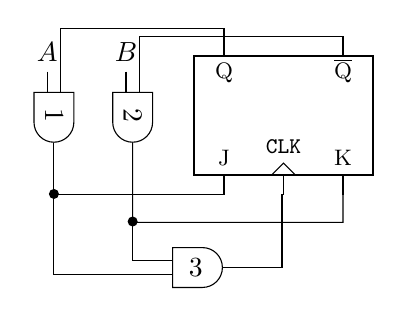
\begin{tikzpicture}[label distance=2mm]
	\node (A) at (0,0) {$A$};
	\node (B) at (1,0) {$B$};
%	\node[not gate US, draw, rotate=-90] at ($(A)+(0.5,-1)$) (NotA) {};
%	\node[not gate US, draw, rotate=-90] at ($(B)+(0.5,-1)$) (NotB) {};
%	\foreach \i in {A,B}{
%		\path (\i) -- coordinate (punt\i) (\i |- Not\i.input);
%		\draw (punt\i) node[branch] {} -| (Not\i.input);}
\node[and gate US, draw, logic gate inputs=nn,rotate=-90,anchor=input 2] at ($(A)+(0,-0.5)$) (gate1) {1};
\node[and gate US, draw, logic gate inputs=nn,rotate=-90,anchor=input 2] at ($(B)+(0,-0.5)$) (gate2) {2};
\node[and gate US, draw, logic gate inputs=nn, anchor=input 1] at ($(gate2.output)+(0.5,-1.5)$) (gate3) {3};
\draw (A) |- (gate1.input 2);
%\draw (NotB) |- (gate1.input 2);
%\draw (NotA) |- (gate2.input 1);
\draw (B) |- (gate2.input 2);

\draw (3,-0.8) node[flipflop JK, rotate=90, scale=0.9, flipflop def={t2={\texttt{CLK}}}](ff1){};

\draw (gate1.input 1) |- ([yshift=0.1cm]ff1.pin 6) -- (ff1.pin 6); % Q
\draw (gate2.input 1) |- (ff1.pin 4); % Qn

\draw (gate1.output)  |- (gate3.input 2);
% \draw (gate1.output) -- ([yshift=-0.5cm]gate1.output) node[above] {} |- (gate3.input 1);
%\draw (gate2.output) -- ([xshift=0.5cm]gate2.output) node[below] {} |- (gate3.input 2);
\draw (gate2.output) |- (gate3.input 1);

%\draw ([xshift=0.4cm]gate1.output) node[branch] {} -| (gate3.input 1);}


\draw (gate3.output) --  ([xshift=0.75cm]gate3.output) node[above] {} |- (ff1.pin 2);
%\draw (gate2.output)  -- ([xshift=2.5cm]gate2.output) node[above] {} |- (ff1.pin 3);	
\draw (gate1.output)  to[short, -*] ([yshift=-0.65cm]gate1.output) node[above] {} |- (ff1.pin 1);

%\draw (gate2.output)  to[short, -*] ([xshift=0.5cm]gate2.output) node[above] {};

\draw (gate2.output)  to[short, -*] ([yshift=-1cm]gate2.output) node[above] {} |- ([yshift=-0.35cm]ff1.pin 3) |- (ff1.pin 3);


% \draw (gate1.output) to[short, -*] ++([xshift=1cm]gate1.output) coordinate(not up);

% \draw (5,0) node[flipflop JK, add async SR]{}; 
%\draw (7,0) node[flipflop JK0]{${FF}_0$};
%\draw (5,0) node[flipflop JK1] (ff1) {};
%\draw (5,0) node[flipflop JK, dot on notQ]{${FF}_1$};

%\draw (5,0) node[flipflop JK, rotate=90, flipflop def={t1=$J_1$,t2={\texttt{CLK}}, t3=$K_1$, t6=$Q_1$, t4=\ctikztextnot{$Q_1$}}](ff1){};


%\node[flipflop DQBR1] (ff0) at (0,3) {${FF}_1$};

%\draw (ff1.pin 2) |- ([xshift=0.7cm]gate1.output);
%\draw ([xshift=0.5cm]gate1.output) |- (ff1.pin 2);

%\draw (4,0) node[cgenerator]{};
 
 	\end{tikzpicture}
 \end{document}
